\section{The Coordinator Pattern}
\label{sec:coordinator}

Most of the topologies of Section~\ref{sec:multi-agent} require a decision on which agent receives a given unit of work, and the literature names the component that takes it differently depending on the topology: supervisor in a centralized topology, manager at any level of a hierarchical topology \cite{zhuLLMBasedMultiAgentOrchestration2026a}. Both perform the same function, so this work fixes one term for it regardless of topology. Table~\ref{tab:coordinator-terms} defines the terminology used from this point on, \emph{coordinator} for the component that takes the decision, \emph{routing} for the decision itself, and \emph{sub-agent} for each specialized agent it can select, together with the synonyms each term replaces. Those synonyms belong to the topology-specific vocabulary of Section~\ref{sec:multi-agent} and to the source it is drawn from \cite{zhuLLMBasedMultiAgentOrchestration2026a}; they are not used elsewhere in this work.

\begin{table}[ht]
	\centering
	\small
	\renewcommand{\arraystretch}{1.4}
	\begin{tabularx}{\textwidth}{@{} l >{\raggedright\arraybackslash}X >{\raggedright\arraybackslash}p{3.1cm} @{}}
		\toprule
		Term & Role & Synonyms \\
		\midrule
		Coordinator & Reads the request, classifies it against the declared sub-agents, and selects exactly one. & Supervisor (centralized topology), manager (hierarchical topology) \\
		Sub-agent & Specialized agent that a coordinator can select; acts under its own instructions and tools once selected. & Worker \\
		Routing & The decision the coordinator takes. & --- \\
		Handoff & The act of passing the request to the selected sub-agent. & --- \\
		Assignment & A handoff in which the sub-agent returns its response to the coordinator, which continues the work. & --- \\
		Delegation & A handoff in which the sub-agent continues on its own and returns the response directly to the requester. & --- \\
		\bottomrule
	\end{tabularx}
	\caption[Terminology used for the coordinator pattern]{Terminology used for the coordinator pattern, and the synonyms the same roles take in the source topology taxonomy \cite{zhuLLMBasedMultiAgentOrchestration2026a}.}
	\label{tab:coordinator-terms}
\end{table}

Correspondingly, the specialized agents of Section~\ref{sec:multi-agent} take the role of sub-agent whenever a coordinator selects among them.

A request enters the system and is read first by the coordinator. The coordinator classifies the request against the sub-agents declared to it and selects exactly one. Passing the request to the selected sub-agent is the \emph{handoff}. Once it happens, the selected sub-agent acts under its own instructions and tools and produces a response. From there, two paths are possible. Figure~\ref{fig:routing-direct} shows \emph{delegation}: the response is returned directly to whoever issued the request, and the coordinator plays no further part once the handoff has been made. Figure~\ref{fig:routing-coordinator} shows \emph{assignment}: the response is returned to the coordinator, which reads it and elaborates the final response that is sent back. In both cases the coordinator selects one sub-agent, which runs and produces the response, while every sub-agent that was not selected is never invoked.

The handoff is exclusive to the sub-agent selected. Other sub-agents at the same level are never invoked and never see the request, even ones that could plausibly have handled it. Nothing in the pattern reopens the selection once it has been made: the request reaches one sub-agent, and the rest of the run proceeds from what that one sub-agent produces.

\begin{figure}[ht]
	\centering
	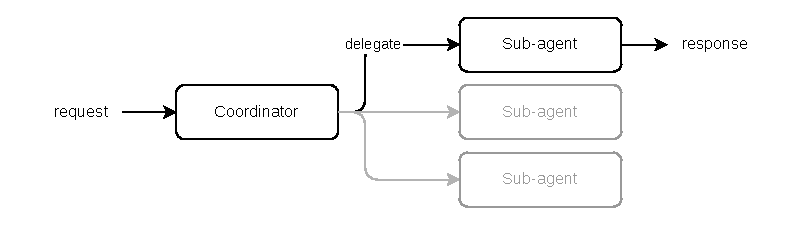
\includegraphics[width=0.9\textwidth]{images/routing_response_direct.pdf}
	\caption[Direct response]{Delegation. The selected sub-agent returns its response straight to the requester; the coordinator does not see it.}
	\label{fig:routing-direct}
\end{figure}

\begin{figure}[ht]
	\centering
	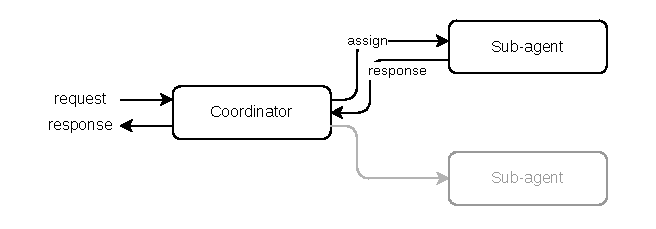
\includegraphics[width=0.74\textwidth]{images/routing_response_coordinator.pdf}
	\caption[Coordinator-mediated response]{Assignment. The selected sub-agent returns its response to the coordinator, which elaborates the final response sent to the requester.}
	\label{fig:routing-coordinator}
\end{figure}

\subsection{Separable and overlapping specialization}
\label{subsec:separable-overlapping}

What the routing decision has to resolve depends on how the sub-agents relate to each other. The sub-agents may cover disjoint subject matter, and in this case the wording of a request separates them. A support system with a billing agent and a shipping agent is of this kind: a request that mentions an invoice or a refund belongs to the billing agent, and a request that mentions a package or a delivery date belongs to the shipping agent. The two agents rarely share vocabulary, so the classification is straightforward from the text alone.

By contrast, in other systems the sub-agents may cover the same subject matter, or subject matters that are closely related. In this case, the wording of a request becomes harder to map to the right one. A travel-booking system with an agent dedicated to the lowest fare and a separate agent dedicated to the shortest travel time is of this kind: both agents can receive a request about the same flight, and the wording of the request might not, by itself, indicate which of the two constraints the requester meant to prioritize.

The same effect is documented in intent classification. ATIS and SNIPS are two datasets of task-oriented dialog utterances. Each utterance is labeled with its \emph{intent class}, the category of goal it expresses, such as \emph{flight} or \emph{airfare} \cite{bihaniFuzzyClassificationMultiintent2021}. Bihani and Rayz compared classification accuracy across the two and reported that it depends on the lexical overlap between the classes \cite{bihaniFuzzyClassificationMultiintent2021}. In ATIS, phrases such as \emph{show me} and \emph{from} repeat across different intent classes; accuracy on it is lower and more variable than on SNIPS, where utterances of different intents share fewer words \cite{bihaniFuzzyClassificationMultiintent2021}. They gave the utterances \emph{show me flights to Philadelphia coming from Baltimore}, labeled as the intent \emph{flight}, and \emph{show me airlines with flights from Denver}, labeled as the intent \emph{airline}, as an example of this overlap \cite{bihaniFuzzyClassificationMultiintent2021}. Higher lexical overlap between the classes lowers the accuracy with which an utterance is mapped to the correct one. This is the same difficulty that a coordinator faces when the sub-agents that it selects among cover overlapping subject matter, as in the fare and travel-time example above.

This extends to multi-turn scenarios. In conversational systems, a request is not necessarily self-contained: the element that fixes which sub-agent should handle it can appear in an earlier turn rather than in the last one. The context relevant to the routing decision is then spread across turns alternated between the user and the assistant, which adds the task of gathering that context to the difficulty of overlapping vocabulary described above.

\subsection{Downstream dependence on the routing decision}
\label{subsec:downstream-dependence}

The coordinator is the causally earliest step of the coordinator pattern described above, and the only one whose output determines which other component runs at all. Once the request has been handed to a sub-agent, no later step reopens the selection. An error made by the coordinator is therefore inherited by everything computed after it. The sub-agent applies its own criteria to a request that should have been handled under different criteria, and its output can be internally consistent while still addressing the wrong problem.

A wrong routing decision is therefore a problem of \emph{trajectory}: the correctness of a run is a property of the whole sequence of steps, and a wrong step early in it is not repaired by anything that follows. It is one instance of a broader problem in evaluating agents, discussed in Chapter~\ref{chap:evaluating-agents}.
